\clearpage
\section{The Experiment}

\subsection{The Large Hadron Collider\label{sec:lhc}}

The Large Hadron Collider (LHC) is a particle accelerator and collider
housed 100 meters undeground in a 27 km long circular tunnel situated 
beneath the Swiss-French border. The collider consists of two 
counter-circulating particle beams which are made to collide at four points 
along the ring. Figure~\ref{fig:lhc} shows the location of the LHC and 
the four main detectors each housed at a different collision point.\\
\indent The machine contains four straight long sections where acceleration, 
collimation, and beam dump systems are housed. The longer arc sections are
in fact comprised of 1232 straight dipole magnets 15 meters in length designed to contain 
the particle beams in a circular path. Each section is held at a 
super-conductive temperature of 2 Kelvin which provides magnetic fields up to 8
Tesla that steer the beams. Higher order multi-pole magnets are 
placed near the interaction points to collimate and align the 
colliding beams. Unwanted beam interaction with residual gas in the beam pipes
is minimized by vacuuming the beam pipes to pressures below $10^{-10}$~mbar.

\begin{figure}[h!]
  \begin{center}
      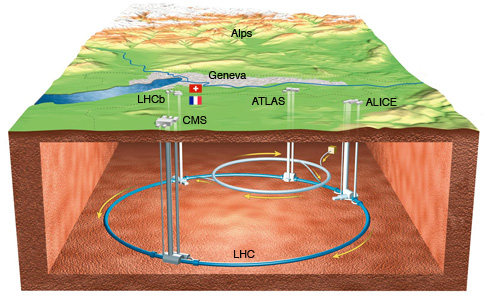
\includegraphics[width=0.40\textwidth,]{figures/CERNMap.jpg}
      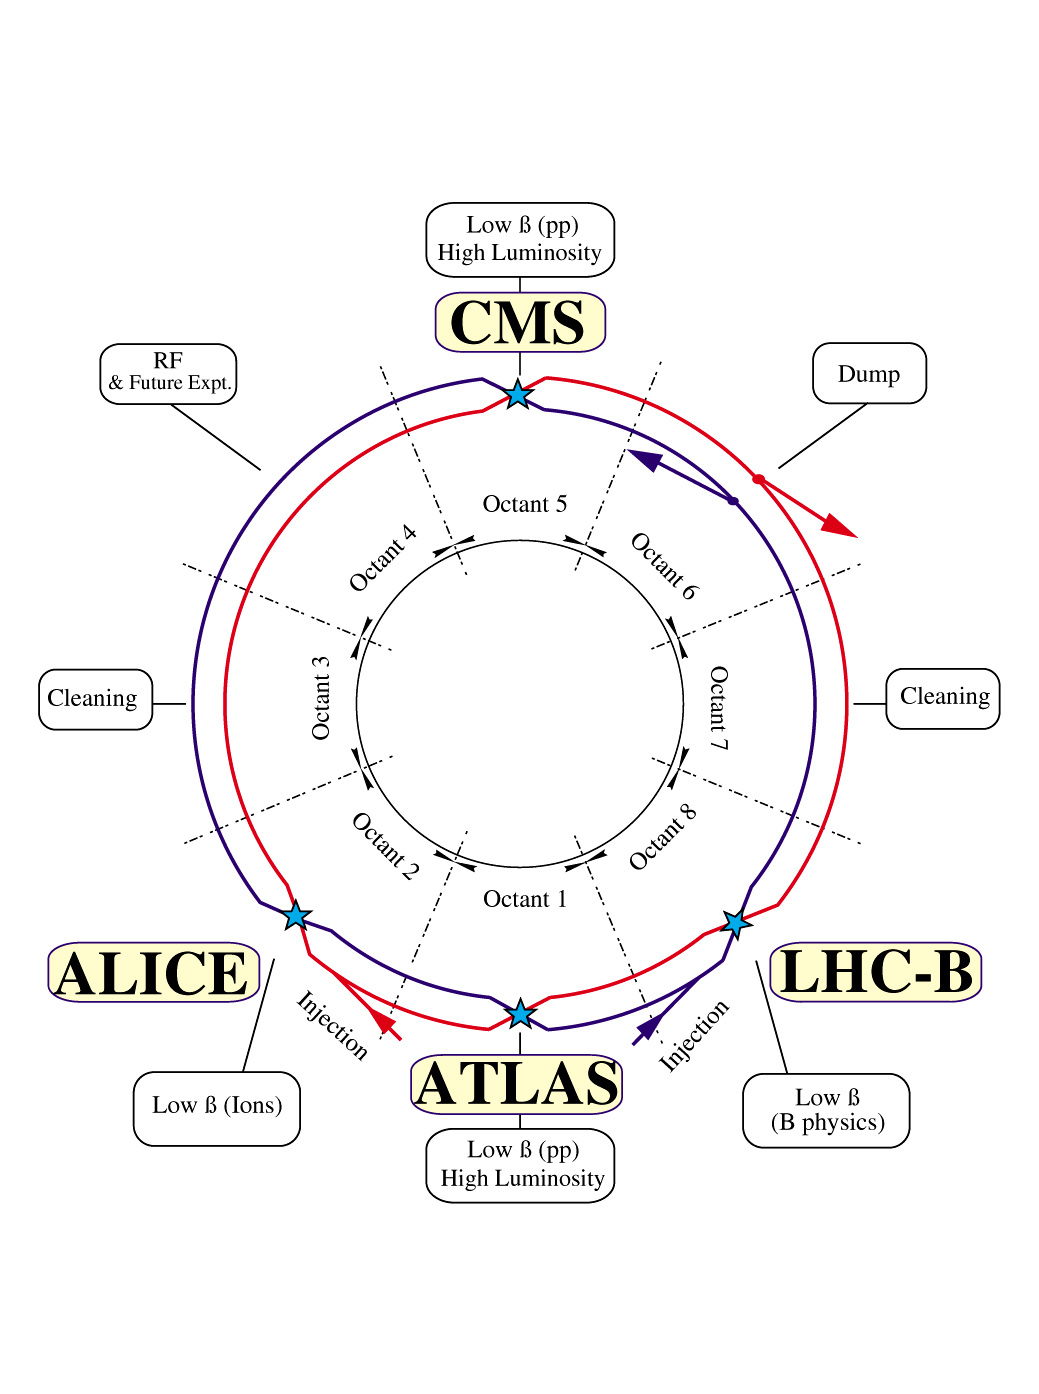
\includegraphics[width=0.35\textwidth,]{figures/lhc-pho-1997-060.jpg}
      \caption{\label{fig:lhc} Left: a geographical map of the location of the LHC. Right: 
      the layout of LHC.}
  \end{center}
\end{figure}

\indent The protons are accelerated along straight sections of the ring where 
Radio-Frequency (RF) cavities generating electromagnetic fields are 
tuned to deliver protons a ‘kick’ of energy at each revolution in the accelerator ring. 
Protons that are ideally timed and have exactly the desired energy, will feel 
a zero accelerating force from the RF cavity, while protons with slightly different 
energies that arrive earlier or later are decelerated or accelerated. As a result, 
the proton beams are divided in discrete ``bunches'' of protons. Each bunch, before collision,
measures $16~\micron$ transversally and $\sim\!\!30$~cm long. Bunches are separated 7~m apart.
The LHC has been designed to operate with 2808 bunches per beam, with about $10^{11}$ protons per bunch. 
The figure of merit for colliders such as the LHC is the luminosity, a quantity 
influencing the rate of collisions. The instantaneous luminosity depends on the number of protons
per beam, the transverse dimensions of the beams (the more the beams are squeezed,
the higher the probability that a proton-proton collision takes place), and the bunch-
crossing frequency. The number of events N of a certain process with cross section σ
produced per second can be expressed as
%
\begin{equation}
  \label{eq:lumi}
  \frac{dN}{dt} = \,\mathcal{L} \times \sigma
\end{equation}
%
The luminosity integrated over the course of the three separate proton-proton collision runs
is shown in Figure~\ref{fig:int_lumi}. 
%The large increases in delivered luminosity in such
%a short time indicates both the phenomenal success of LHC commissioning and running, and 
%the challenge presented to CMS to accommodate new running conditions nearly continuously, 
%in particular to design and deploy suitable trigger tables, readout thresholds, 
%reconstruction algorithms, and analysis methods.

\begin{figure}[h!]
  \begin{center}
      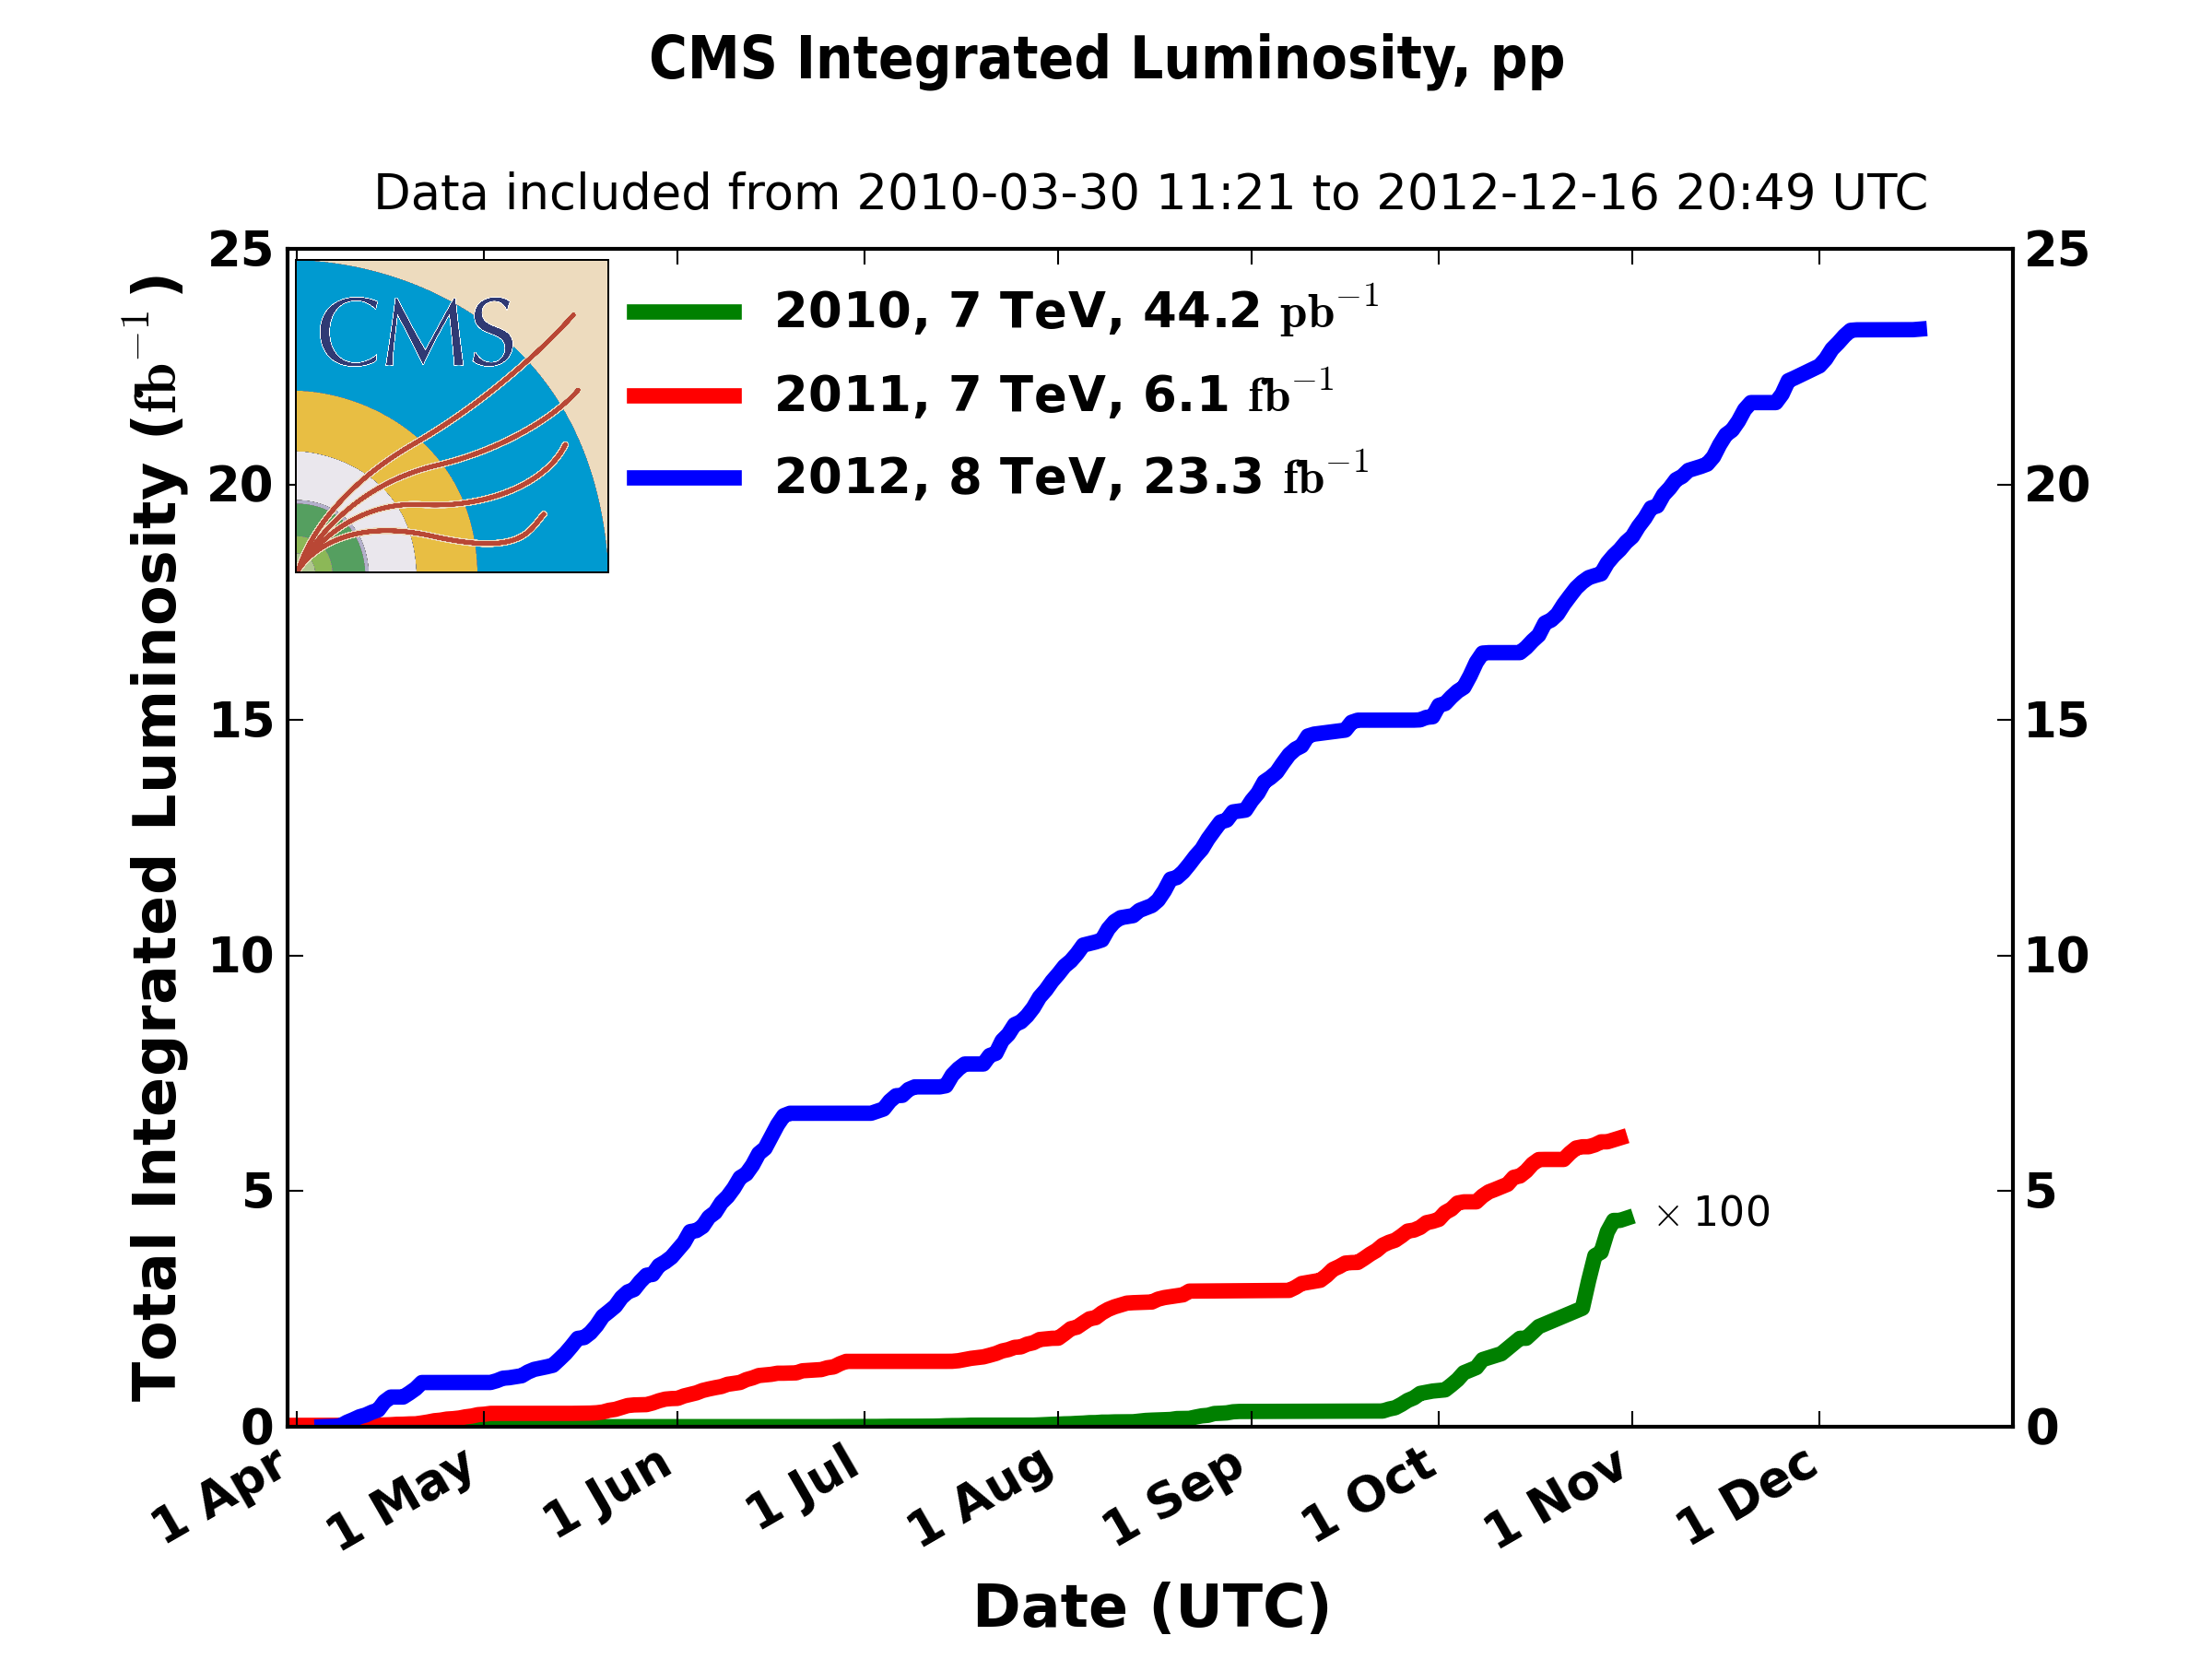
\includegraphics[width=0.53\textwidth,]{figures/int_lumi_cumulative_pp_2.png}
      \caption{\label{fig:int_lumi} The luminosity integrated over the course of the three 
      separate proton-proton collision runs as recorded by CMS.  
      Note: the 2010 curve is multiplied by 100 for legibility.}
  \end{center}
\end{figure}

\FloatBarrier
\subsubsection{High energy proton collisions}
\cite{green2005high}
Despite collision bunches each containing $10^{10}$ protons, the number of collisions
between protons average to only around 20 per bunch crossing. Of these collisions only
one or two have substantial momentum transfer to produce energetic elementary 
particles, the rest produce soft jets who's energies are eventually substracted from the event's
reconstructed objects. In a proton collision, the interaction actually takes place between the 
constituent quarks and gluons and the distributions of what fraction of a proton's momentum a 
constituent gluon or quark carries are given by parton distribution functions (PDFs). \\
\indent For a particular production process, e.g. $pp \ra \ttbar$ or $pp \ra \bar{g}\bar{g}$, there are 
various parton scattering processes, e.g. from initial gg or $q\bar{q}$, which contribute; their cross sections 
are integrated over momentum fraction according to the PDFs and summed to obtain a total production cross section.
Results of such cross section computations for a variety of processes are shown
in Figure~\ref{fig:crossSec}.

\begin{figure}[h!]
  \begin{center}
      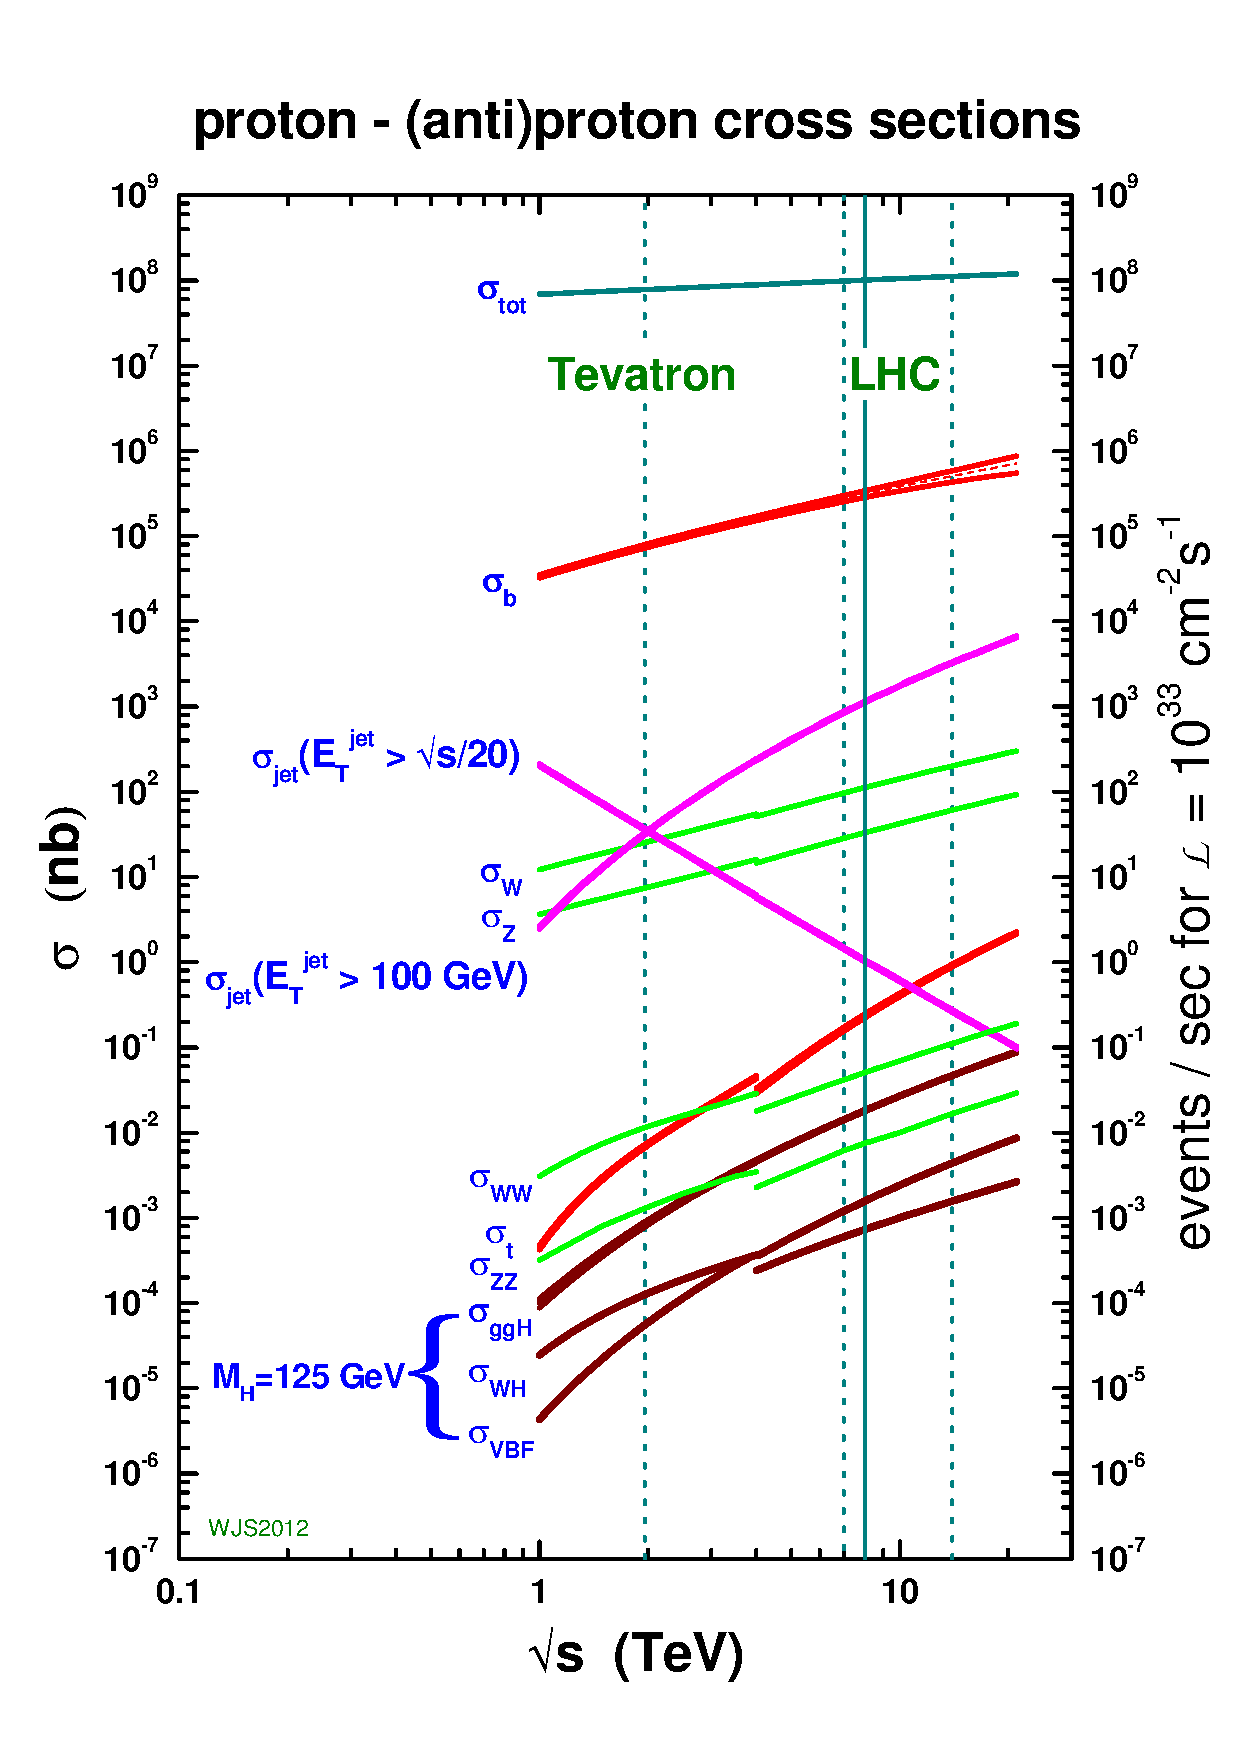
\includegraphics[width=0.40\textwidth,trim=0 2cm 0 0]{figures/crosssections2012_v5}
      %      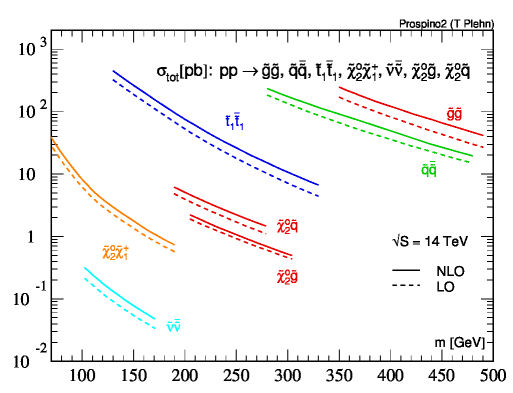
\includegraphics[width=0.40\textwidth,]{figures/PEacs.png}
      \includegraphics[width=0.5\textwidth, ]{figures/nlonll_lhc8_tpformat.eps}
      \caption{\label{fig:crossSec} Left: the cross sections (in nb) of various SM processes vs. center-of-mass
              energy in $pp$ collisions when $\sqrt{s}>1$~\TeV, from Ref.~\cite{stirling-xs}. Right: 
              The cross sections (in pb) of various SUSY processes vs. sparticle for $pp$ collisions
              at $\sqrt{s}=8$~\TeV. From Ref.~\cite{Beenakker:1996ed}.} 
  \end{center}
\end{figure}

The various SUSY production cross sections drive the choice of interpretation 
of the results for this search, and this is further discussed in Section~\ref{sec:signature}. 
The small SUSY cross sections compared with that of known processes highlight 
the challenge for the search.\\
\indent Given that the energy of the colliding quarks or gluons is not known on 
an event-to-event basis, the use of conservation of total energy is not possible. 
The different momentums of the two colliding partons give a ``boost'' to the center-of-mass 
of the scattering system along the beam line which varies event-by-event. On the other hand, 
the component transverse to the beam axis of the momentum of the colliding quark or gluon is 
known to be zero. Therefore it is convenient to discuss jets (as well as other reconstructed 
particles) in terms of these quantities: transverse momentum $\pt$, which is invariant under 
such boosts, or similarly transverse energy $\equiv E \sin\left(\theta\right)$, with 
$0 \leq \theta \leq \pi$ where $\theta$ is the polar angle from the beam-line; and pseudo-rapidity:

\begin{equation}
        \eta \equiv −\ln\left( \tan\left(\theta/2\right)\right),
        \label{pseudo}      
\end{equation}

of which differences remain invariant. Furthermore, it is convenient to describe the distance between
objects in the detector as:

\begin{equation}
        R \equiv \sqrt{\left(\Delta\phi\right)^2 + \left(\Delta\eta\right)^2},
        \label{pseudo}      
\end{equation}

where the azimuthal angle $\phi$ is the angle sweeping around the beam-line.

\subsection{The Compact Muon Solenoid detector\label{sec:cms}}

\subsubsection{The detector}
The Compact Muon Solenoid (CMS) is a multi-purpose detector designed to reconstruct
the visible products of the colliding particles of the LHC. It's first name refers to 
the its compact design; it packs twice the weight in $1/6^{th}$ the volume of ATLAS, 
the other multi-purpose detector at CERN. Its second name refers to the detector's design
to measure muons with great precision; with the ability to resolve a muon's $\pt$ down to 
1\% in some cases. It's last name refers to to the superconducting solenoid of diameter 
6~m and length 12.5~m. When ramped up to 18~kA, it prodcues a magnetic field of 3.8~T providing
a means of measuring kinematic properties of charged particles. The magnet is kept at a 
superconducting temperature of 4.8 Kelvin. The dectector is segmented into a ``barrel'' 
section, flanked on each side by an ``endcap''. The fact that the tracking and calorimeter 
instrumentation is located in the magnet bore lends to the detector's compact design. 
CMS nearly completely encloses the interaction point of the two beams, and provide an 
accurate measurment of global transverse momentum imbalance of a collision event. The 
layout is shown in the bottom plot of Figure~\ref{fig:cms}. The detector is described in 
full detail in Ref.~\cite{1748-0221-3-08-S08004,Bayatian:922757,Bayatian:942733}, but a brief
overview is given below. 

\begin{figure}[h!]
  \begin{center}
      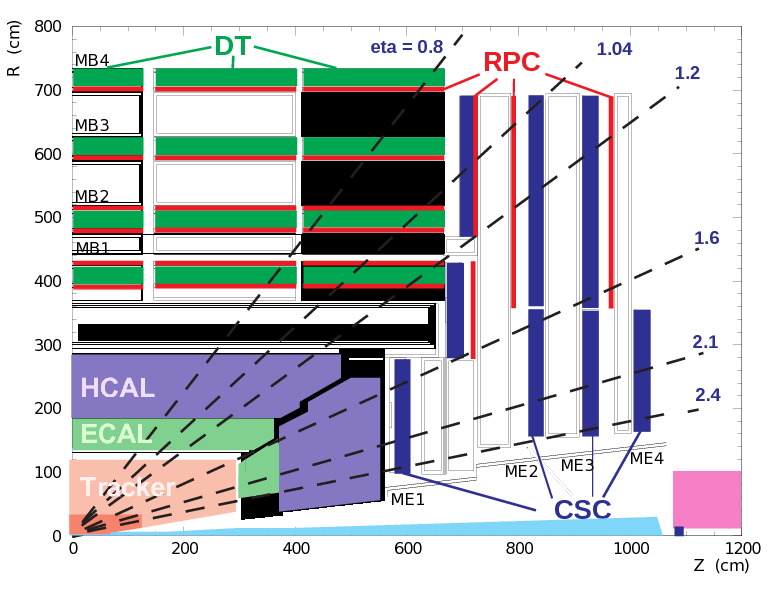
\includegraphics[width=0.65\textwidth, trim = 2cm 0 0 0]{figures/cmsQuad.png}\\
      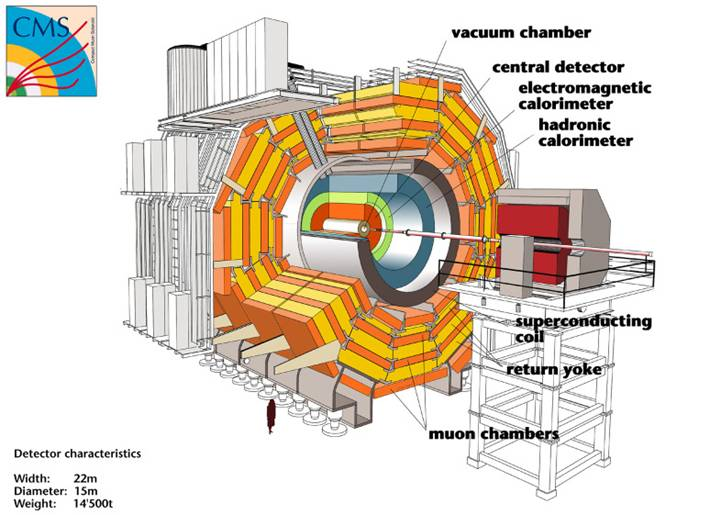
\includegraphics[width=0.65\textwidth,]{figures/CMS_Detector.jpg}
      \caption{\label{fig:cms} Top: a view of one quadrant of CMS. The volume enclosing 
      the tracker is shown in light red, the electromagnetic calorimeter in light green, 
      the hadron calorimeter in lavender, and the forward calorimeter in magenta. 
      The muon detectors are labeled, from Ref.~\cite{2012JInst...7P0002T},
      Bottom: a perspective view of CMS from Ref.~\cite{1748-0221-3-08-S08004}.}
  \end{center}
\end{figure}

The closest subdetector to the beam is the tracker. Charged particles are tracked in 
3 dimensions within a distance of 4.4~cm up to 10~cm from the beam axis with three concentric layers of hybrid 
pixel detectors totaling 66 million pixels. Two additional layers shaped in disks are placed at each 
end the of the barrel giving the pixel detector coverage up to pseudo-rapidity $|\eta| < 2.5$.
Leaving the pixel detector, particle continue through 10 barrel layers and 12 endcap disks 
of the silicon strip tracker extending to 1.1~m from the beam axis. The silicon strip tracker
consists of 10 million strips covering a total area $200~\texttt{m}^2$.  This tracking system
provides high transverse-momentum ($\pt$) resolution, efficiency, and primary- and secondary-vertex
resolutions.\\
\indent Surrounding the tracker is the electromagnetic calorimeter (ECAL) consisting of over 60 thousand scintillating 
lead tungstate crystals in the barrel ($|\eta| < 1.48$) and a further 7,500 crystals in each endcap extending
the coverage up to each measuring $|\eta| < 2.5$. The crystals have a front-face cross section
of approximately $22 \times 22~\texttt{mm}^2$ (resp. $28.6 \times 28.6~\texttt{mm}^2$) in the barrel (resp. endcap) with a
length of 23~cm corresponding to $\sim25$ radiation lengths, i.e. the length which an electron loses
all but $1/e$ of its energy or $7⁄9$ of the mean free path for pair production by a high-energy photons.  
Avalanche photo-diodes detect the scintillated light in the barrel $(|\eta| < 1.479)$ vacuum photo-triodes 
in the endcap $(1.479 < |\eta| < 3.0)$. For extra spatial precision, the ECAL also contains lead-silicon 
sampling detector that sit in front of the endcaps. These allow CMS to distinguish between single high-energy 
photons and close pairs of low-energy photons.\\
\indent Surrounding ECAL is the hadronic calorimeter (HCAL), which measures a particle’s position, 
energy and arrival time using alternating layers of brass absorber and plastic fluorescent scintillator.
It is divided into two hemisphere composing the barrel section and two endcap covering $|\eta| < 3.0$. 
The light from the scintillators is summed up over the layers and segmented into 
``towers'' of area $\Delta\eta \times \Delta\phi = 0.087 \times 0.087$ for $|\eta| < 1.6$, 
and approximately $0.17 \times 0.17$ for $|\eta| > 1.6$. These summed optical signals are converted 
into fast electronic signals by photosensors called Hybrid Photodiodes (HPDs). When lights hit the 
light sensitive photocathode in the HPD, it is converted into electrons which are accelerated across 
a gap of a few millimeters onto a silicon diode target. The target is divided up into 19 pixels each 
of which can generate its own amplified electronic signal and allows the detection and amplification 
of up to 19 separate calorimetry signals with one HPD. The electronic signals are then sampled for 
each collision and digitized using special HCAL-designed integrated circuits called QIE chips (Charge 
Integration and Encode) and sent to the trigger and data acquisition system for analysis.
Outside of the endcaps are forward calorimeters (HF) extending the coverage of HCAL to $|\eta| = 5.0$ 
and thereby improving the hermicity of CMS. The HF is made of steel absorber and radiation-hard
quartz fibers which detect Cherenkov light from relativistic particles. The hit-occupancy is sampled
during each beam crossing to provide instantaneous luminosity measurements for the LHC. The luminosity
is also provided in larger time granularity called ``lumi sections'' which consist a period of
218 beam orbits or about 23 seconds~\cite{CMS-PAS-SMP-12-008}.\\ 
\indent Muons are measured in the range  $|\eta| < 2.4$ with instrumentation interlaced between the magnet's
return yoke as shown in Figure~\ref{fig:cms}. Three types of technologies are used depending
on pseudo-rapidity: drift tubes ($|\eta| < 1.2$), cathode strip chambers ($0.9 < |\eta| < 2.4$), and
resistive-plate chambers ($|\eta| < 1.6$). The first two technologies provide a precise position measurement 
and trigger, whilst the third one provides precise timing information, as well as a second independent 
trigger mechanism. \\
\indent Recording each collision event would require storing 40 Terabytes per second of data, which
is simply impossible. A trigger system which decides which event to be recorded is implemented in 
two parts: ``Level One'' (L1), and ``High Level'' (HLT). The L1 Trigger is implemented largely in 
programmable electronics and is designed to operate at 40 MHz and reduce the rate of 
accepted events to 100 kHz. It consists of three steps: In the first step, the
``trigger primitive'' generator sums up the transverse energy from an ECAL or HCAL trigger
tower. Then the regional calorimeter trigger determines regional electrons/photons bits and isolation. 
Lastly, the global calorimeter trigger can combine this information and
calculate more complex observables using all of the calorimeter. In parallel, a second chain
triggers muons. 
The HLT is a reconstruction and decision software system implemented to reduce the incoming 
L1 stream of accepted events to $\mathcal{O}$(100~Hz). The software is built to reconstruct
events as closely as possible to offline reconstruction given the constraints on processing time
of around 50 ms per event. Difference between online and offline reconstructed objects can 
introduce trigger inefficiencies in an analysis, this is further discussed in the 
context of the triggers and objects used in this analysis in Section~\ref{sec:signal_triggers}.\\
\indent Events passing the trigger selection chain are duplicated and stored in raw format at
the CERN computing center, where a final offline reconstruction is performed. Events passing
a common type of trigger are stored in a dataset and copied to many CMS computing sites around the
globe for storage and analysis. 
  
\subsubsection{Event reconstruction\label{sec:eventReco}}

As detector instrumentation vary greatly througout a particle's path, reconstruction
of an event and its objects relies on various stragies and algorithms. Yet the common goal 
remains the same throughout: to reconstruct, from raw detector information,
higher-level objects which represent as best as possible properties of: individual
particles, groups of particles e.g. jets, or global event variables e.g. total energy
recorded. The following gives an overview of the reconstruction sequence relevent for this search
while many detais of the reconstruction technique can be found in Ref.~\cite{Bayatian:922757,Bayatian:942733}. 

\begin{figure}[h!]
  \begin{center}
      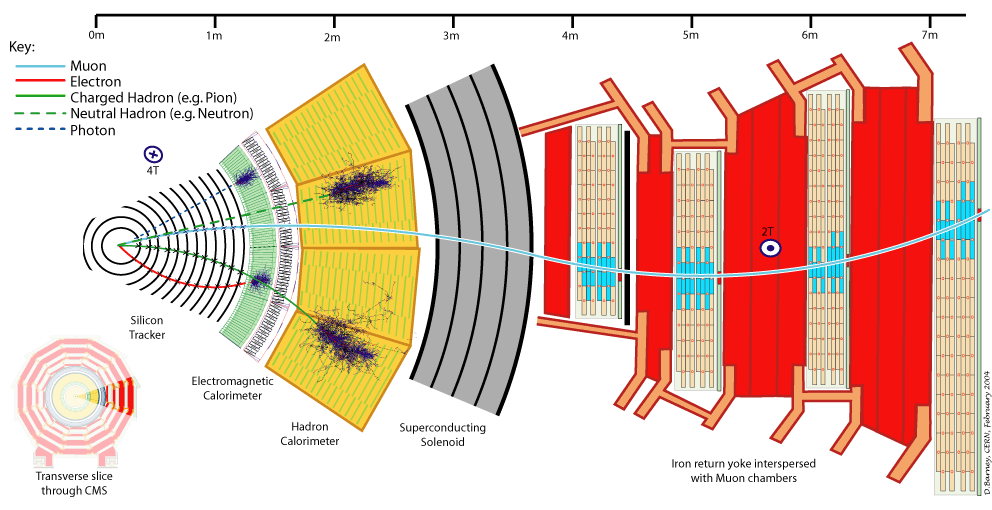
\includegraphics[width=.9\textwidth,]{figures/CMS_Slice}
      \caption{\label{fig:cmdSlice} }
  \end{center}
\end{figure}

%\indent The raw data read out from CMS are first converted to software representations
%of the digital samples of the detector signals, which are associated with individual
%detector elements. In a typical procedure, knowledge of pulse shapes, time-dependent
%channel-by-channel baseline values and gains, and detector geometry is then used to
%convert these samples into reconstructed ``hits'', i.e. energy deposits in particular
%detector locations at particular times.\\


\indent The collection of tracks left by charged particles in the tracker during an events are 
reconstructed using an iterative process. The inital iteration searches for tracks 
that are easiest to find (e.g., of relatively large $\pt$, and produced near the 
interaction region). After each iteration, hits associated with tracks are removed, 
thereby reducing the combinatorial complexity, and simplifying subsequent iterations 
in a search for more difficult classes of tracks (e.g., low-$\pt$, or greatly displaced
tracks)~\cite{Chatrchyan:2014fea}. Each iteration follows similar steps: (a) a seed 
track is generated from a few hits to be used as the initial estimate for the track's 
trajectory parameters and uncertainties; (b) the seed track is extrapolated along the 
expected flight path of a charged particle, searching for additional hits that can be 
assigned to the track candidate thereby making it more precise; (c) a final fit is performed 
using all of track its hits. The reconstructed tracks are then clustered on the basis of 
their z-coordinates at their point of closest approach the beam-line and fitted to determine 
the position of the vertex. This clustering allows for the reconstruction of any number 
of proton-proton interactions in the same LHC bunch crossing.\\
\indent In the standard CMS muon reconstruction, tracks are first reconstructed independently 
in the inner tracker (tracker track) and in the muon system (standalone-muon 
track)~\cite{1748-0221-7-10-P10002}. Then, for each standalone-muon track, a matching tracker 
track is found by comparing parameters of the two tracks propagated onto a common surface. A 
fit to the combined hits of the two subdetectors is performed to obtain a muon referred to as 
a ``global muon''. This and other approaches are described in Ref.~\cite{PAS-MUO-10-002}. The 
quality criteria on the reconstruction and identification of muons for this analysis are 
discussed in Section~\ref{sec:muonReco}. \\
\indent Photons and electrons can be reconstructed through their energy deposit in the ECAL. 
For instance, single photons impinging at the center of a crystal deposit about 97\% of their 
incident energy in a cluster of crystals 5 $\times$ 5 in $\eta-\phi$ space~\cite{Bayatian:922757}. 
But the situation is in general more complicated for the average electron, as they bend while 
passing through the tracker under the influence of the mangetic field and radiate photons through 
bremsstrahlung. Clustering algorithm are therefore designed to take into account their spread of 
hits in $\phi$ and collect the bremsstrahlung energy. The average cluster size from electrons end 
up being 5 crystals in $\eta$ by 35 in $\phi$ in the barrel, or one or more group of 5 by 5 
crystals in the endcaps. The crystals with the highest deposited energy are matched with nearby 
hits in the tracker layer which seed a dedicated radiative loss model to build the electron track.\\
\indent Jets are reconstructed using the anti-kt algorithm~\cite{antikt} set to sequentially clusters 
particle tracks or energy deposits within a cone of radius R=0.5. The input to the algoritm define
the jet type; two types of jets are studied in the analysis calorimeter (calo) jets and Particle-Flow 
(PF) jets the are defined below.\\
\indent Calorimeter jets are reconstructed using energy deposits in the ECAL and HCAL which are 
combined into calorimeter towers as inputs. A calorimeter tower consists of one or more HCAL cells 
and the geometrically corresponding (ECAL) crystals.\\
\indent The Particle Flow (PF) algorithm aims to reconstruct, identify and calibrate each individual 
particle in the event by combining the information from all CMS sub-detector systems. PF particles are 
reconstructed as a combination of charged particle tracks and clusters in the electromagnetic 
and hadronic calorimeters, as well as signals in either of the two CMS pre-shower detectors 
and the muon system. Depending on which of the detector systems contribute to a single particle, 
it is identified as either an electron (track+ECAL), muon (track+ECAL+HCAL+Muon System), photon (ECAL), 
charged hadron (track+ECAL+HCAL), or neutral hadron (HCAL). The algorithm employs strategies to handle 
ambiguities stemming from overlapping detector signals to avoid information double-counting. Based on 
the particle type, the energy of each particle is calibrated. Charged hadrons are treated under the 
assumption that they are pions. As a result of the PF reconstruction, the inputs to the jet clustering 
are almost fully calibrated and the resulting higher level objects (jets) require small a posteriori 
energy corrections~\cite{Chatrchyan:2011ds}.\\
\indent The relative simplicity of calo-jet reconstruction allows for fast computational time while 
the complexity of PF-jets reconstruction provides better angular and $\pt$ resolutions. This search 
uses calo-jets in the HLT trigger algorithm and PF-jets in the offline analysis; the consequences are 
discussed in Section~\ref{signal_triggers}. The relative $\pt$ resolution for central jets for both 
jet types determined using dijet $\pt$-asymmetry, is shown in Figure~\ref{fig:jetRes}. 

\begin{figure}[h!]
  \begin{center}
  \subfigure[]{
      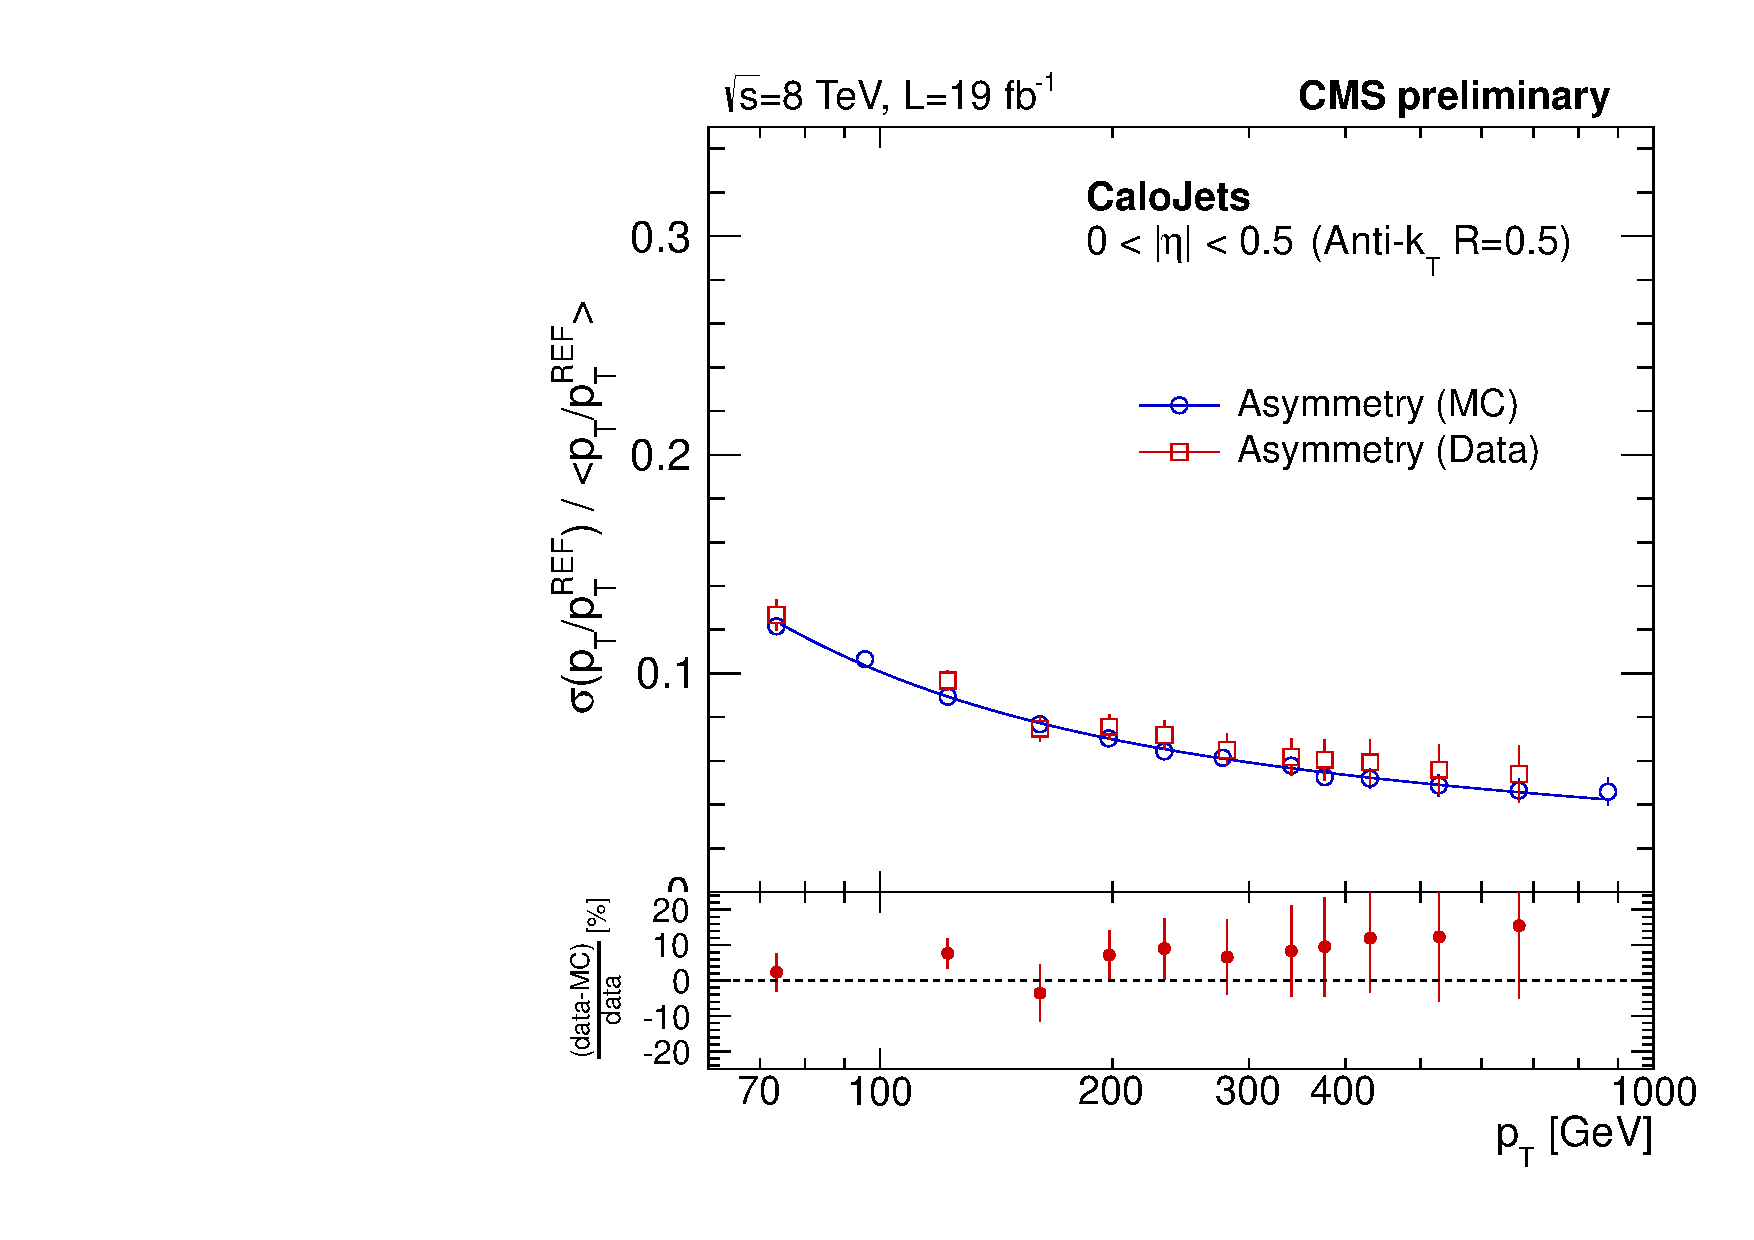
\includegraphics[width=0.45\textwidth,]{figures/ak5calo_relRes}}
      \subfigure[]{
      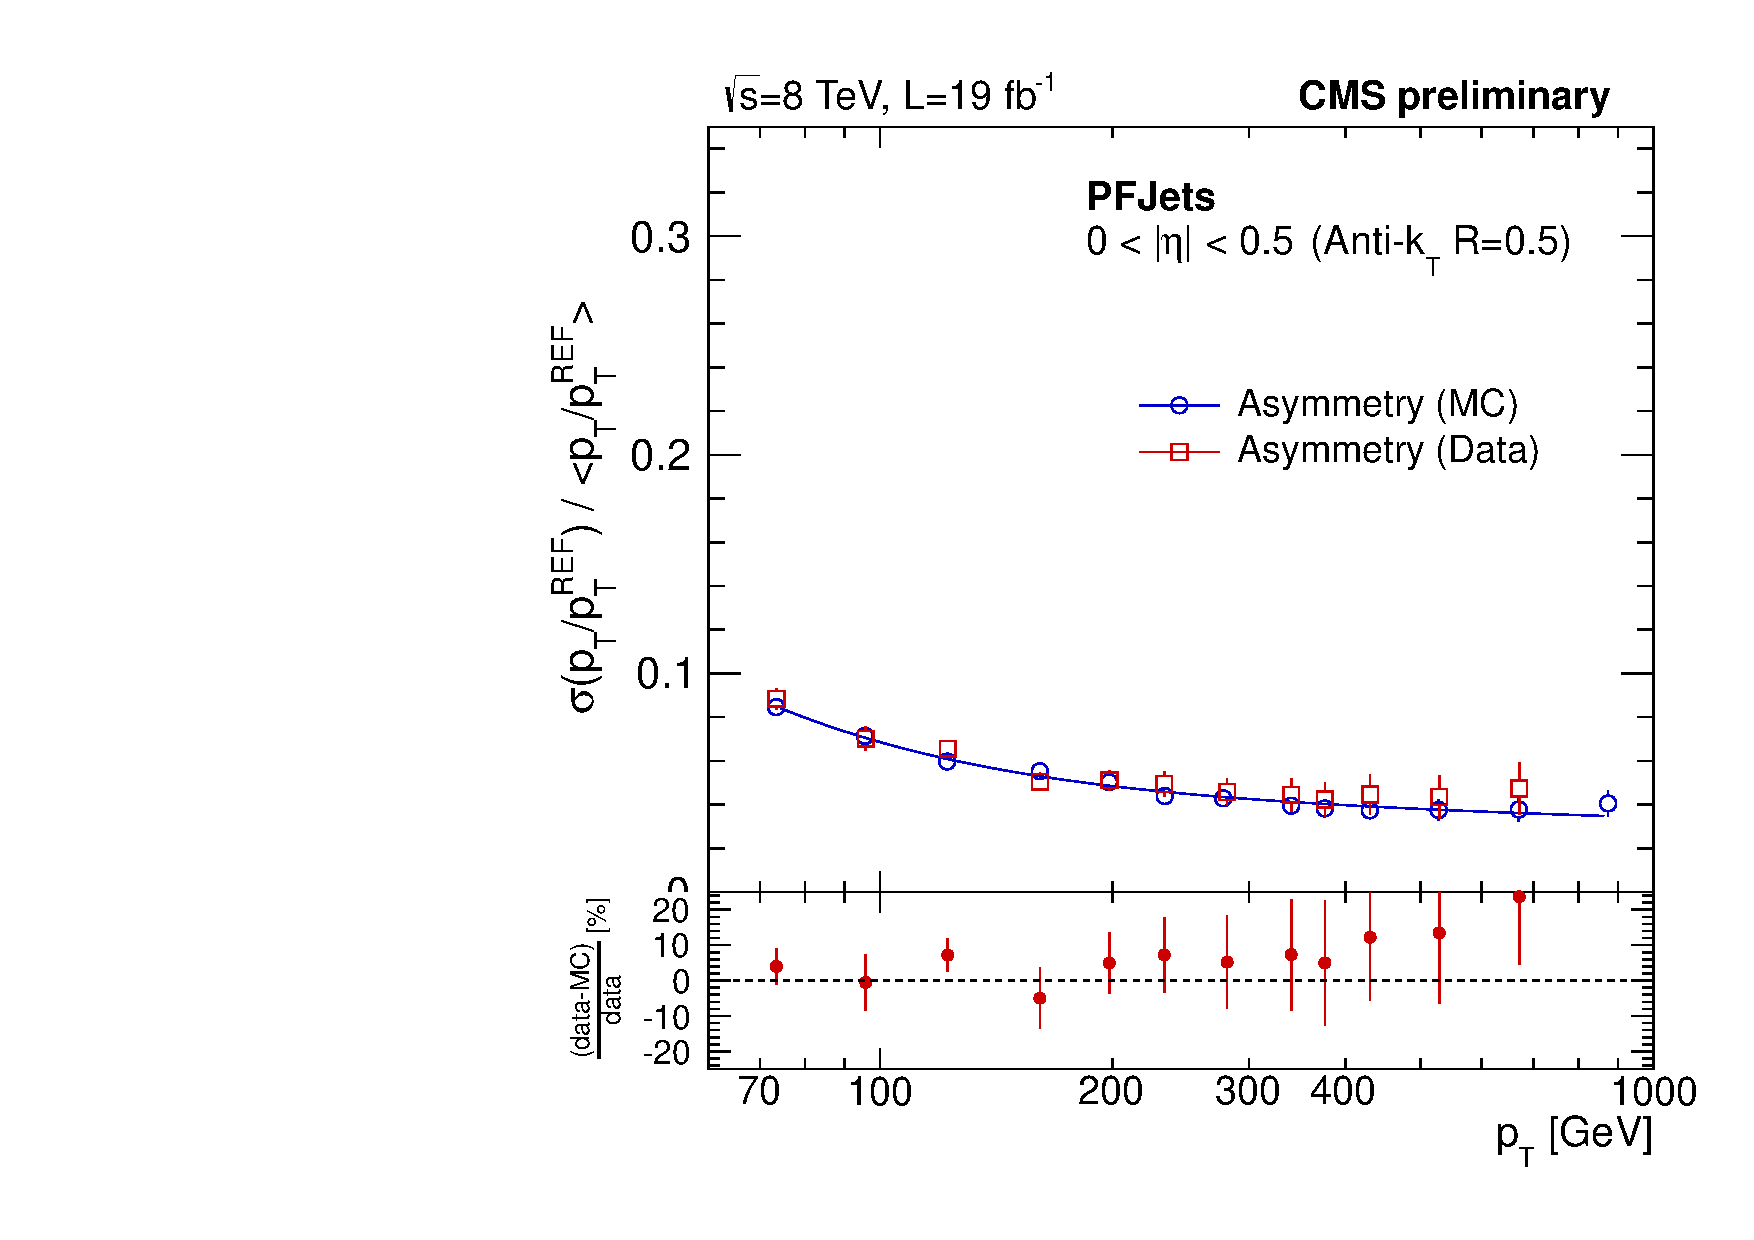
\includegraphics[width=0.45\textwidth,]{figures/ak5pf_relRes}}
      \caption{\label{fig:jetRes} The relative $\pt$ resolution as a function of jet $\pt$
              for calo jets (a) and PF jets (b) in the center of the barrel using the dijet
              $\pt$-asymmetry method~\cite{CMS-PAS-JME-10-014}.}
  \end{center}
\end{figure}

%Missing transverse energy (\met) is computed from the same towers of energy deposits 
%in the calorimeters that are used for jet-finding; it is the negative of the vectorial
%sum of their components transverse to the beam-axis. Corrections are applied to
%accommodate the jet energy corrections and the presence of muons~\cite{1748-0221-6-09-P09001}.
%
